\documentclass[conference]{IEEEtran}
\usepackage{graphicx}
\usepackage{booktabs}
\usepackage{amsmath}
\usepackage{cite}
\graphicspath{{../Results/real_fields/}}

\begin{document}

\title{SAR and Optical Feature Fusion for Crop Classification Using YieldSAT}

\author{\IEEEauthorblockN{Het Patel (AU2440266), Dhairya Shah (AU2440128), Jay Daftari (AU2440271), Hiya Soni (AU2440084)}
\IEEEauthorblockA{ECE 501 Digital Image Processing, Project 19, Group 3\\
Ahmedabad University\\
Code: github.com/Het1236/DIP\_2026\_19\_3}}

\maketitle

\begin{abstract}
This report describes the first half of our project on crop classification using optical and SAR satellite images together. We use the YieldSAT dataset for Argentina and Brazil. It gives Sentinel-2 optical images and crop labels but no radar data. We build a pipeline that removes clouds from the optical time series. The pipeline then makes one clean composite per field and computes vegetation indices. We download Sentinel-1 radar data for the same fields through Google Earth Engine. We reduce speckle with a Lee filter and align the radar image to the optical grid. We checked all 1302 fields in the dataset. We also ran the full pipeline on three real fields, one for each crop. The Lee filter reduced the VV noise by about 20 percent and kept the mean unchanged. Feature fusion and classification are planned for the second half.
\end{abstract}

\begin{IEEEkeywords}
crop classification, SAR, optical, Sentinel-1, Sentinel-2, speckle, YieldSAT
\end{IEEEkeywords}

\section{Introduction}
Knowing which crop grows in a field helps with farm planning and food security. Satellites can map crops over large areas. Optical satellites measure sunlight reflected from the ground. Their images are easy to read but clouds block the view. Radar satellites send their own signal and work through clouds. Their images are noisy and harder to read. Using both kinds of data together may give better crop maps than using either one alone.

Our project studies this idea. We extract classical hand-crafted features from optical and SAR images of the same field. We then fuse the features and train a classical machine learning model. The project asks us to compare optical-only, SAR-only and fused results. We do not use deep learning.

We use the YieldSAT dataset \cite{yieldsat}. Our group was assigned Argentina and Brazil. This mid-semester report covers the data and the processing pipeline for both image types. We check the real data for all 1302 fields and build an optical pipeline. We also build a Sentinel-1 pipeline and test everything on three real fields.

\begin{figure*}[t]
\centering
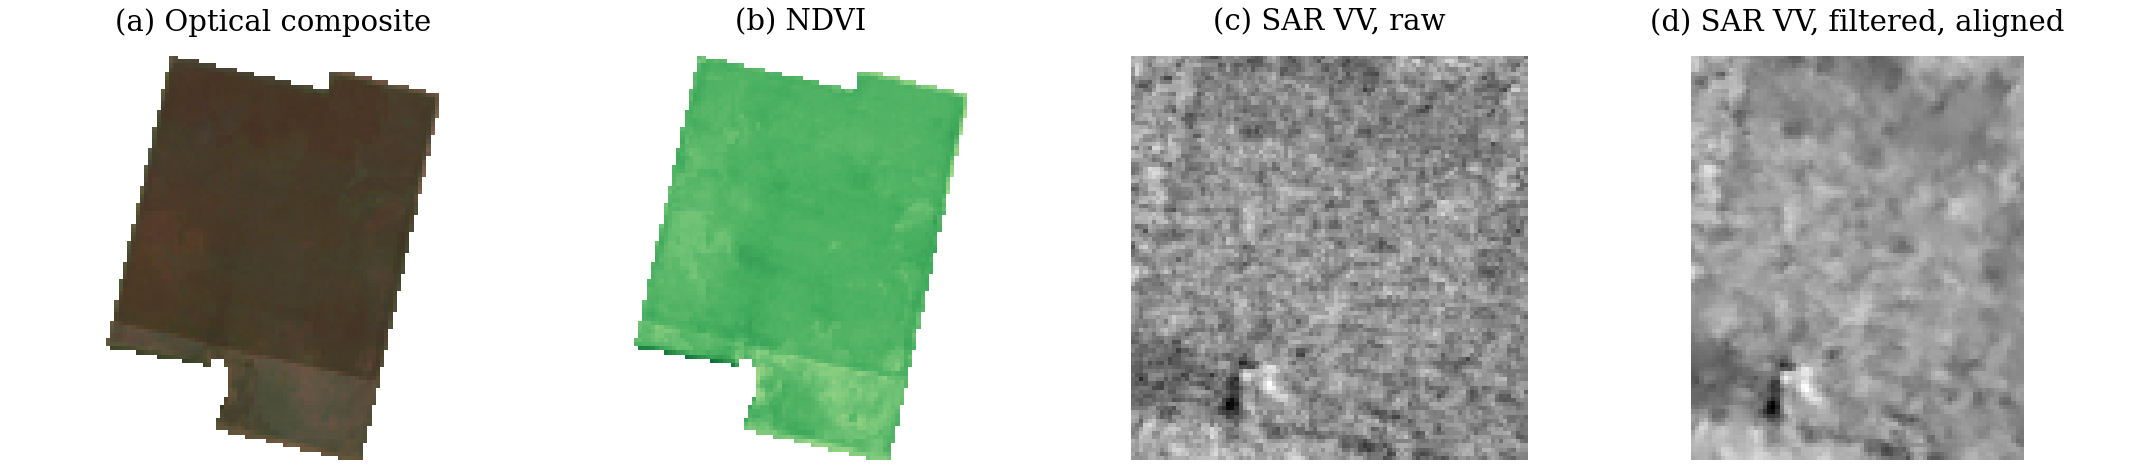
\includegraphics[width=\textwidth]{report_corn_field.png}
\caption{Real corn field in Argentina. (a) Cloud-free optical composite. (b) NDVI. (c) Sentinel-1 VV as downloaded. (d) VV after the Lee filter and alignment to the optical grid.}
\label{fig:corn}
\end{figure*}

\section{Methodology}
The pipeline has an optical branch and a SAR branch. Both work on the same field and give images on the same grid.

\subsection{Dataset}
YieldSAT has 751 fields for Argentina and 551 for Brazil. Each field is a folder. It holds Sentinel-2 images for every date between seeding and harvest. Each image has 12 bands at 10~m resolution. A second file for each date holds the scene classification layer (SCL). A metadata file gives the crop label, the seeding and harvest dates and the UTM zone. Pixel values are stored as 16-bit integers. We divide them by 10000 to get reflectance. The value 0 means no data. YieldSAT has no SAR data, so we download it ourselves.

\subsection{Optical processing}
The SCL gives a class for every pixel. We keep classes 4, 5, 6 and 7. These are vegetation, bare soil, water and unclassified. We drop every other class. These include cloud, cloud shadow, snow and no data. A date is dropped when fewer than 20\% of the field pixels are usable. For each pixel the composite is the median of the valid dates:
\begin{equation}
C(x,y,b)=\operatorname*{median}_{t\in T(x,y)} I_t(x,y,b)
\end{equation}
Here $T(x,y)$ is the set of valid dates at that pixel and $b$ is the band. We use the median because one missed cloud pixel affects it less than it affects the mean.

From the blue, green, red and near-infrared (NIR) bands we compute four indices \cite{rouse}. The first two are
\begin{equation}
\mathrm{NDVI}=\frac{\mathrm{NIR}-\mathrm{Red}}{\mathrm{NIR}+\mathrm{Red}}
\end{equation}
\begin{equation}
\mathrm{EVI}=2.5\,\frac{\mathrm{NIR}-\mathrm{Red}}{\mathrm{NIR}+6\,\mathrm{Red}-7.5\,\mathrm{Blue}+1}
\end{equation}
The other two are GNDVI and NDWI. They use the green band in place of red.

\subsection{SAR processing}
We query Sentinel-1 GRD scenes in interferometric wide mode with VV and VH polarization \cite{sentinel1} through Google Earth Engine \cite{gee}. The search area is the exact extent of the field raster. The date range runs from the seeding date to the harvest date of that field. We take the median of all scenes and download it at 10~m in decibels.

SAR images contain speckle. This is a grainy noise caused by the radar waves interfering with each other. We apply a Lee filter \cite{lee} with a $5\times5$ window to each band:
\begin{equation}
\hat I=\bar I+k\,(I-\bar I),\qquad k=\frac{\sigma_w^2}{\sigma_w^2+\overline{\sigma_w^2}}
\end{equation}
Here $\bar I$ and $\sigma_w^2$ are the mean and variance in the window. The term $\overline{\sigma_w^2}$ is the average window variance over the image. In flat areas $k$ is small and the pixel moves toward the local mean. Near edges $k$ is large and the pixel is mostly kept.

Finally we resample the filtered SAR image onto the pixel grid of the YieldSAT field with bilinear interpolation. After this an optical pixel and a SAR pixel cover the same ground area.

\section{Results}
\subsection{Dataset check}
We scanned every field folder. All 751 Argentina fields and 551 Brazil fields loaded without errors. The crop counts match the YieldSAT paper. Argentina has 185 corn, 440 soybean and 126 wheat fields. Brazil has 118 corn, 293 soybean and 140 wheat fields. We found one problem. The image is a rectangle but the field is not. The corners outside the field have SCL class 0. Our first mask let these pixels through. We fixed this by keeping only the usable classes listed above.

\subsection{Three real fields}
We ran the full pipeline on one Argentina field for each crop. The optical composite uses the whole season from seeding to harvest. Table~\ref{tab:fields} shows the field means. Fig.~\ref{fig:corn} shows the corn field.

\begin{table}[t]
\caption{Pipeline output for one real field per crop.}
\label{tab:fields}
\centering
\footnotesize
\setlength{\tabcolsep}{3pt}
\begin{tabular}{lccccc}
\toprule
Crop & Dates kept & S1 scenes & NDVI & VV (dB) & VH (dB)\\
\midrule
Corn    & 52/96 & 15 & 0.52 & $-10.23$ & $-17.50$\\
Soybean & 47/81 & 12 & 0.41 & $-9.44$  & $-16.81$\\
Wheat   & 49/93 & 14 & 0.48 & $-14.90$ & $-22.22$\\
\bottomrule
\end{tabular}
\end{table}

\subsection{Speckle filtering}
We tested the Lee filter on a real Sentinel-1 composite of a farmland area in Argentina. It had 112 by 113 pixels and used 5 scenes. The standard deviation of VV fell from 1.35~dB to 1.08~dB. This is a drop of about 20\%. The mean stayed at $-12.87$~dB. Panels (c) and (d) of Fig.~\ref{fig:corn} show the same effect on the corn field.

\section{Discussion}
The cloud mask keeps about 55\% of the dates for each field. This leaves enough clear images to build a composite. The VV minus VH difference is close to 7.3~dB for all three fields. This is stable and suggests the SAR download and filtering work correctly.

The wheat field has a much lower VV value than the other two. It is also from a different season. The wheat was planted in June and harvested in November 2023. The corn and soybean fields were planted in October and November and harvested in March and April. The season or the crop structure may explain the difference. We have only one field per crop so we cannot draw a firm conclusion.

The NDVI values are low because the composite mixes early growth with later stages. A composite from the peak of the season should give higher values. We also tested only three fields from one country and used only field means so far.

\section{Conclusion}
We built and tested the data pipeline for both image types on real YieldSAT and Sentinel-1 data. The optical branch gives a clean composite and four indices. The SAR branch gives a filtered image aligned to the optical grid. Next we will use a peak-season window and add texture features from the gray level co-occurrence matrix \cite{haralick}. We will then build a feature table for many fields. Random Forest and SVM models will be trained on optical-only, SAR-only and fused features. We will report accuracy, F1-score and confusion matrices.

\begin{thebibliography}{9}
\bibitem{yieldsat} M. Miranda \textit{et al.}, ``YieldSAT: A multimodal benchmark dataset for high-resolution crop yield prediction,'' in \textit{Proc. IEEE/CVF Conf. Computer Vision and Pattern Recognition (CVPR)}, 2026, arXiv:2604.00940.
\bibitem{sentinel1} R. Torres \textit{et al.}, ``GMES Sentinel-1 mission,'' \textit{Remote Sens. Environ.}, vol. 120, pp. 9--24, 2012.
\bibitem{gee} N. Gorelick \textit{et al.}, ``Google Earth Engine: Planetary-scale geospatial analysis for everyone,'' \textit{Remote Sens. Environ.}, vol. 202, pp. 18--27, 2017.
\bibitem{lee} J.-S. Lee, ``Digital image enhancement and noise filtering by use of local statistics,'' \textit{IEEE Trans. Pattern Anal. Mach. Intell.}, vol. PAMI-2, no. 2, pp. 165--168, Mar. 1980.
\bibitem{rouse} J. W. Rouse \textit{et al.}, ``Monitoring vegetation systems in the Great Plains with ERTS,'' in \textit{Proc. 3rd ERTS Symp.}, NASA SP-351, 1974, pp. 309--317.
\bibitem{haralick} R. M. Haralick, K. Shanmugam, and I. Dinstein, ``Textural features for image classification,'' \textit{IEEE Trans. Syst., Man, Cybern.}, vol. SMC-3, no. 6, pp. 610--621, Nov. 1973.
\end{thebibliography}

\end{document}
